\newpage
\section{Gewichtbasiertes Lernen}
\subsection{Notationen}
\begin{flushleft}

\begin{align*}
x^{(i)} &= \text{Die Features des i-ten Samples} \\
x_{j}^{(i)} &= \text{Der Wert des j-ten Features im i-ten Samples} \\
m &= \text{Die Anzahl Samples} \\
n &= \text{Die Anzahl Features} \\
X &= \text{Datenset} \\
y &= \text{Target Vektor}
\end{align*}

In der Regel ist ein Datenset als Matrix $X$ gegeben mit $\mathbb{R}^{m \times n}$


\begin{center}
	\begin{table}[h]
	\begin{tabular}{|c|c|c|c|c|}
		\hline
		\textbf{Feature 1} & \textbf{Feature 2} & \textbf{...} & \textbf{Feature n} & \textbf{Target} \\ 
		\hline
		$x_{1}^{(1)}$ & $x_{2}^{(1)}$ & ... & $x_{n}^{(1)}$ & Klasse X  \\ 
		\hline
		$x_{1}^{(2)}$ & $x_{2}^{(2)}$ & ... & $x_{n}^{(2)}$ & Klasse Y  \\ 
		\hline
		$x_{1}^{(m)}$ & $x_{2}^{(m)}$  & ... & $x_{n}^{(m)}$  & Klasse Z  \\ 
		\hline
	\end{tabular}
\end{table}
\end{center}


\end{flushleft}



% === PERCEPTRON ===
\newpage
\subsection{Perceptron}
\begin{flushleft}

                        
Das Perceptron ist ein linearer binärer Klassifikator. In einem Lernprozess generiert das Perceptron eine lineare Funktion, welche Daten in zwei Gruppen unterteilen kann. Eine Gruppe wird oberhalb der Funktionsgeraden liegen, die andere unterhalb.

Eine Konstante (1) wie auch der Feature-Vektor werden individuell mit Gewichten multipliziert und addiert. Ist die Summe grösser als 0, so werden die Input-Features der Klasse 1 zugeordnet. Anderenfalls der Klasse 0.

Für zwei Features $x_{1}$ und $x_{2}$ würde die lineare Funktion wie folgt lauten:
$$w_{0} + x_{1}w_{1} - x_{2}w_{2} = 0$$
                        
                        
\newcommand{\myThresholdFunction}{
\draw[thick] %(-2.25em,0em) -- (1.25em,0em) 
			 (-0.5em,1.25em) -- (-0.5em,-1.25em)
(-0.5em,1.25em) -- (0.5em,1.25em)
(-0.5em,-1.25em) -- (-1.5em,-1.25em)
;}


\begin{figure}[H]
\centering
\label{fig:perceptron}
\begin{tikzpicture}[
     % define styles 
     clear/.style={ 
         draw=none,
         fill=none
     },
     net/.style={
         matrix of nodes,
         nodes={ draw, circle, inner sep=10pt },
         nodes in empty cells,
         column sep=2cm,
         row sep=-9pt
     },
     >=latex
]
% define matrix mat to hold nodes
% using net as default style for cells
\matrix[net] (mat)
{
% Define layer headings
|[clear]| \parbox{1.3cm}{\centering Input\\layer} & 
|[clear]| \parbox{1.3cm}{\centering Gewichtete\\Summe} &
|[clear]| \parbox{1.3cm}{\centering Schwellwert\\Funktion} \\
         
$+1$  		& |[clear]| & |[clear]| \\
|[clear]| 	& |[clear]| & |[clear]| \\
$x_{1}$  	& |[clear]| & |[clear]| \\
|[clear]| 	& $\Sigma$  & \myThresholdFunction \\
\vdots  	& |[clear]| & |[clear]| \\
|[clear]| 	& |[clear]| & |[clear]| \\
$x_{n}$  	& |[clear]| & |[clear]| \\
};
\draw[->] (mat-2-1) -- node[above=1mm] {$w_{0}$} (mat-5-2);
\draw[->] (mat-4-1) -- node[above=1mm] {$w_{1}$} (mat-5-2);
\draw[->] (mat-6-1) -- node[above=1mm] {$\vdots$} (mat-5-2);
\draw[->] (mat-8-1) -- node[above=1mm] {$w_{n}$} (mat-5-2);
\draw[->] (mat-5-2) -- node[above=1mm] {$\hat{y}$} (mat-5-3);
\draw[->] (mat-5-3) -- node[right=2em] {$\begin{cases}
       		1 & \text{wenn } \hat{y} \geq 0, \\
       		0 & \text{sonst.}
    	\end{cases}$} +(2cm,0);
\end{tikzpicture}
\caption{Perceptron als Model}
\end{figure}


Die Entscheidungsfunktion $d$ entscheidet zu welcher Klasse ein gegebener Inputvektor gehört.

\begin{align*}
w_{i}\cdot x &= \hat{y} \\
d(\hat{y}) &= \begin{cases}
       		1 & \text{wenn } \hat{y} \geq 0, \\
       		0 & \text{sonst.}
    	\end{cases} \\
d(w_{i} \cdot x) &= \begin{cases}
       		1 & \text{wenn } \hat{y} \geq 0, \\
       		0 & \text{sonst.}
    	\end{cases} \\
d(w_{i}^{T}x) &= \begin{cases}
       		1 & \text{wenn } \hat{y} \geq 0, \\
       		0 & \text{sonst.}
    	\end{cases} \\
\end{align*}


Im Gegensatz zu vielen anderen gewichtsbasierten Lernalgorithmen werden beim Perceptron die Gewichte \textbf{nur dann aktualisiert, wenn die vorhergesagte Klasse falsch war.}

Definitionen

\begin{align*}
\Delta w_{j}  &= \text{Gewichtsupdate} \\
\hat{y}^{(i)} &= \text{Vorhergesagter (berechneter) Zielwert} \\
y^{(i)} &= \text{Effektiver Zielwert (Label)} \\
\eta &= \text{Learning Rate} \\
(y^{(i)} - \hat{y}^{(i)}) &= \text{Errorfunktion} \\
\end{align*}

Gewichte werden zu Beginn zufällig initialisiert und dann jeweils wie folgt angepasst:
$$w_{j} \coloneqq w_{j} + \Delta w_{j}$$
$$\Delta w_{j} = \eta (y^{(i)} - \hat{y}^{(i)}) x_{j}^{(i)}$$

Im Falle von zwei Input Features, sähe das Aktualisieren der Gewichte so aus:
\begin{align*}
\Delta w_{0} &= \eta (y^{(i)} - \hat{y}^{(i)}) \\
\Delta w_{1} &= \eta (y^{(i)} - \hat{y}^{(i)}) x_{1}^{(i)} \\
\Delta w_{2} &= \eta (y^{(i)} - \hat{y}^{(i)}) x_{2}^{(i)} \\
\end{align*}



% === LERNEN ===
\newpage
\subsubsection{Lernen}
Wir betrachten nun ein Beispiel wie das Perceptron lernt. Die Gewichte werden zufällig wie folgt initialisiert:

\begin{align*}
	 w_{0} &= -0.5\\
	 w_{1} &= 2 \\
	 w_{2} &= -1 \\
\end{align*}

Die Lernrate $\eta$ setzen wir auf $0.5$.
Wir betrachten den Punkt $P_{0} = (3,5)$, welcher der Klasse 0 angehört und berechnen dessen $\hat{y}$.
\begin{align*}
\hat{y} &= w \cdot x \\
		&= -0.5 + 2*3 - 5 \\
		&= 0.5
\end{align*}

Gemäss der Schwellwertfunktion ist der Punkt $P_{0}$ fälschlicherweise der Klasse 1 zugehörig. Daher werden die Gewichte angepasst.

\begin{align*}
\Delta w_{j} &= \eta (y^{(i)} - \hat{y}^{(i)}) x_{j}^{(i)} \\
\Delta w_{0} &= 0.5(0-0.5) \\
			 &= -0.25 \\
\Delta w_{1} &= 0.5(0-0.5)3 \\
			 &= -0.75 \\
\Delta w_{2} &= 0.5(0-0.5)5 \\
			 &= -1.25\\
\end{align*}

Wir passen nun die Gewichte entsprechend an.

\begin{align*}
	 w_{0} &= w_{0} + \Delta w_{0}\\
	 	   &= -0.5 + (-0.25) \\
	 	   &= -0.75 \\
	 w_{1} &= w_{1} + \Delta w_{1} \\
	 	   &= 2 + (-0.75) \\
	 	   &= 1.25 \\
	 w_{2} &= w_{2} + \Delta w_{2} \\
	 	   &= -1 + (-1.25) \\
	 	   &= -2.25 \\
\end{align*}

Diese Grafik zeigt die Perceptron Funktion vor und nach dem ersten Lern-Update. Für den zweiten Punkt (Klasse 1) in der Grafik, würde die Gewichte nicht aktualisiert werden, da dieser bereits korrekt klassifiziert werden würde.


\begin{figure}[H]
	\centering
	\label{fig:perceptron_learning}
	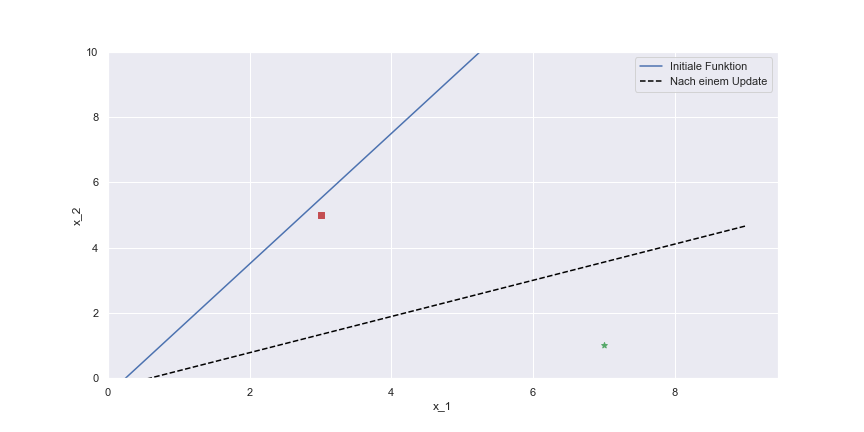
\includegraphics[scale=0.6]{figures/perceptron_learning}
	\caption{Perceptron Lernbeispiel}
\end{figure}




% =======
\newpage
\subsubsection{Vorhersagen}
Im folgenden Beispiel würde sich beispielsweise die Gerade $3x_{1} - x_{2} - 9 = 0$ als Entscheidungsfunktion ergeben. Dies ergibt die Gewichte:
\begin{align*}
	 w_{0} &= -9\\
	 w_{1} &= 3 \\
	 w_{2} &= -1 \\
\end{align*}



Wir betrachten einen Punkt $P_{1} = (5,4)$, eingesetzt in die Entscheidungsfunktion $d$:

\begin{align*}
\hat{y} &= w_{i}\cdot x \\
		&= -9 + 3*5 - 4 \\
		&= 2 \\
d(\hat{y}) &= \begin{cases}
       		1 & \text{wenn } \hat{y} \geq 0, \\
       		0 & \text{sonst.}
       		\end{cases} \\
d(2) &= \text{Klasse 1} \\
\end{align*}

\begin{figure}[H]
	\centering
	\label{fig:perceptron_prediction}
	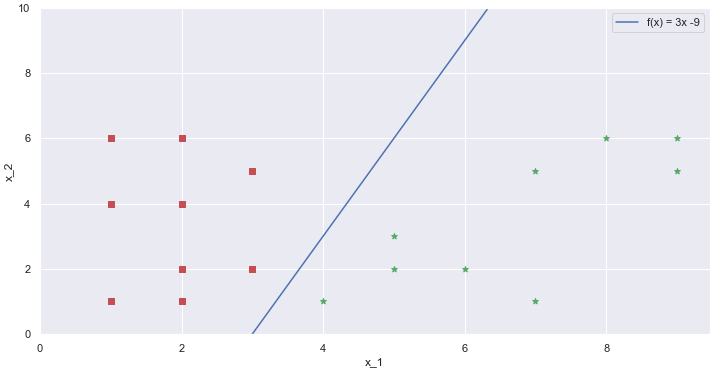
\includegraphics[scale=0.5]{figures/perceptron_line}
	\caption{Perceptron Vorhersage}
\end{figure}

Anhand des Punktes $P_{2} = (2,8)$ zeigen wir, dass das Perceptron auch direkt als Ungleichung angesehen werden kann. Wenn die Ungleichung erfüllt wird, wird der Punkt der Klasse 1 (grüner Stern) zugeordnet. Falls nicht der Klasse 0 (rotes Quadrat)

$$w_{i}\cdot x \geq 0$$
$$ -9 + 3*2 - 8\geq 0$$
$$ -11 \ngeq 0$$

Der Punkt $P_{2}$ wird also der Klasse 0 zugeordnet.

\end{flushleft}

\subsubsection{One-vs-all}
TODO

\newpage
\subsection{Adaline}
\begin{flushleft}
\end{flushleft}

\subsection{Interpretation}
\begin{flushleft}
\end{flushleft}




